% !TeX spellcheck = en_GB
%
\documentclass[presentation]{beamer}
\mode<presentation>{\usetheme{AMSCesenaPurpleAndGold}}
\setbeamertemplate{bibliography item}{\insertbiblabel}
%%%%%%%%%%%%%%%%%%%%%%%%%%%%%%%%%%%%%%%%%%%%%%%%%%%%%%%%%%%%%%%%%%%%%%%%%%%%%%%%
\usepackage[english]{babel}
\usepackage[utf8]{inputenc}
%
\usepackage{SCO-EXTRAAMAS-2021-talk}

%%%%%%%%%%%%%%%%%%%%%%%%%%%%%%%%%%%%%%%%%%%%%%%%%%%%%%%%%%%%%%%%%%%%%%%%%%%%%%%%
\title[\gridex]{
    % same title of the presented paper
	\gridex: An Algorithm for
	\\
	Knowledge Extraction from Black-Box Regressors
}
%
% \subtitle{Extended Abstract}
%
% same authors order of the presented paper
\author[F. Sabbatini et al.]{
	\emph{Federico Sabbatini} % empth the presenting author
	\and 
	Giovanni Ciatto
	\\
	Andrea Omicini
}
%
\institute[UniBo]{
    Dipartimento di Informatica -- Scienza e Ingegneria (DISI)
    \\
    \textsc{Alma Mater Studiorum} -- Università di Bologna
    \\
    \texttt{
        \{\emph{f.sabbatini}, giovanni.ciatto, andrea.omicini\}@unibo.it % emph the presenting author's email
    }
}
%
\date[EXTRAAMAS, 2021]{
	3\textsuperscript{rd} International Workshop on EXplainable and
	\\
	TRAnsparent AI and Multi-Agent Systems (EXTRAAMAS)
	\\
	May 3, 2021, London, UK (online)
}
%%%%%%%%%%%%%%%%%%%%%%%%%%%%%%%%%%%%%%%%%%%%%%%%%%%%%%%%%%%%%%%%%%%%%%%%%%%%%%%%
\AtBeginSection[]
{
%\\\\\\\\\\\\\\\\\\\\\
\begin{frame}<beamer>[c,noframenumbering]
\frametitle{Next in Line\ldots}
\tableofcontents[sectionstyle=show/shaded,subsectionstyle=hide]
\end{frame}
%\\\\\\\\\\\\\\\\\\\\\
}
\AtBeginSubsection[]
{
%\\\\\\\\\\\\\\\\\\\\\
\begin{frame}<beamer>[shrink,noframenumbering]
    \frametitle{Focus on\ldots}
	\mbox{~}
	\tableofcontents[currentsubsection,sectionstyle=shaded,subsectionstyle=show/shaded]
	\mbox{~}
\end{frame}
%\\\\\\\\\\\\\\\\\\\\\
}
%%%%%%%%%%%%%%%%%%%%%%%%%%%%%%%%%%%%%%%%%%%%%%%%%%%%%%%%%%%%%%%%%%%%%%%%%%%%%%%%
\begin{document}
%%%%%%%%%%%%%%%%%%%%%%%%%%%%%%%%%%%%%%%%%%%%%%%%%%%%%%%%%%%%%%%%%%%%%%%%%%%%%%%%

%\\\\\\\\\\\\\\\\\\\\\
\frame{\titlepage}
%\\\\\\\\\\\\\\\\\\\\\

%===============================================================================
\section{Motivation \& Context} % non il contrario?
%===============================================================================

%\\\\\\\\\\\\\\\\\\\\\
\begin{frame}[c]{Context}
    
    %
    \vfill
    %
    \begin{itemize}
        \item ML-based predictors are more and more used in a wide range of fields to perform different tasks
        %
        \begin{itemize}
            \item[e.g.] pattern detection, image and speech recognition, clustering, classification and regression
        \end{itemize}
        
        \vfill
        
        \item predictors hiding their internal logic are named \emph{black boxes}
        %
        \begin{itemize}
            \item[!] black-box predictors cannot give to the user intelligible outputs or \alert{explanations about their outcomes}
        \end{itemize}
        
        \vfill
        
        \item there are critical applications where the output interpretability is not an option
        %
        \begin{itemize}
        	\item for instance healthcare, finance, etc.
        \end{itemize}
    
    	\vfill
        
        \item[$\Rightarrow$] knowledge extraction mechanisms are required to use black-box models in these critical areas 
        
    \end{itemize}
\end{frame}
%\\\\\\\\\\\\\\\\\\\\\

%\\\\\\\\\\\\\\\\\\\\\
\begin{frame}[c]{Motivation}
	Several methods were developed to extract knowledge from black-box predictors, however:
    %
    \vfill
    %
    \begin{itemize}
        \item most of the algorithms existing in the literature focus exclusively on classification tasks, neglecting regression
        %
        \begin{itemize}
            \item[e.g.] \textsc{Trepan}\ccite{Craven1996}, Rule-extraction-as-learning\ccite{craven1994using}, etc.
        \end{itemize}
        
        \vfill
        
        \item most of the knowledge extraction methods applicable to regression black boxes are strongly constrained
        %
        \begin{itemize}
            \item[e.g.] \textsc{RefAnn}\ccite{setiono2002extraction}, only applicable to ANNs with a single hidden layer
        \end{itemize}
        
        \vfill
        
        \item other procedures may suffer of degrading performance when applied to complex problems
        %
        \begin{itemize}
			\item[e.g.] 
			\iter\ccite{huysmans2006iter} as the number of input features grows
		\end{itemize}
        
    \end{itemize}
\end{frame}
%\\\\\\\\\\\\\\\\\\\\\

%\\\\\\\\\\\\\\\\\\\\\
\begin{frame}{Some state of the art}
	
    \begin{itemize}
    	\item ML-based predictors detect patterns and relationships in the data
    	\begin{itemize}
    		\item their acquired knowledge can be reused in similar applications
    	\end{itemize}
    
    	\vfill
    
    	\item However, their knowledge is not explicitly represented
    	\begin{itemize}
    		\item[$\Rightarrow$] lack of interpretability, models described as black boxes\ccite{Lipton2016}
    		\item[$\Rightarrow$] need of more interpretable predictors\ccite{Rudin2019}, inspection techniques\ccite{Guidotti2018}    		
    	\end{itemize}
    
    	\vfill
    	
    	\item[!] \alert{A system is defined \emph{interpretable} if its operations and outcomes can be easily understood by a human being}\ccite{agentbasedxai-extraamas2020}
    	
    	\vfill
    	
    	\item \iter\ccite{huysmans2006iter} is a knowledge-extraction algorithm for black-box regressors
    	\begin{itemize}
    		\item[!] pedagogical method: no constraints on the model nature and structure
    		\item it extracts lists of if-then-else rules by analysing the input feature space 
    		\item global approximation of the underlying black-box regressor 	
    		\item[!] it may be unable to cover the whole input space with its rules   
    		\item[!] prediction discretisation: \iter assigns a constant value to each rule
    		\item inability to handle categorical features, only real-valued ones
    	\end{itemize}
    \end{itemize}

\end{frame}
%\\\\\\\\\\\\\\\\\\\\\

%\\\\\\\\\\\\\\\\\\\\\
\begin{frame}{Contribution of the paper}

\begin{block}{The new \gridex algorithm extends \iter}
    \begin{itemize}
    	\item inheriting its core concepts
    	\item overcoming its major drawbacks
    	\begin{itemize}
    		\item[e.g.] non-exhaustivity and focus on low-importance input regions
    	\end{itemize}
        \item producing shorter rule lists
        \item retaining higher performance
    	\begin{itemize}
			\item predictions w.r.t. the data
			\item fidelity w.r.t. the underlying black box			
		\end{itemize}        
    \end{itemize}
\end{block}

\end{frame}
%\\\\\\\\\\\\\\\\\\\\\

%===============================================================================
\section{\gridex design}
%===============================================================================

%\\\\\\\\\\\\\\\\\\\\\
\begin{frame}%[allowframebreaks]
\frametitle{\iter basic idea}
	\begin{columns}[t]
		\column{0.51\linewidth}
			\centering
			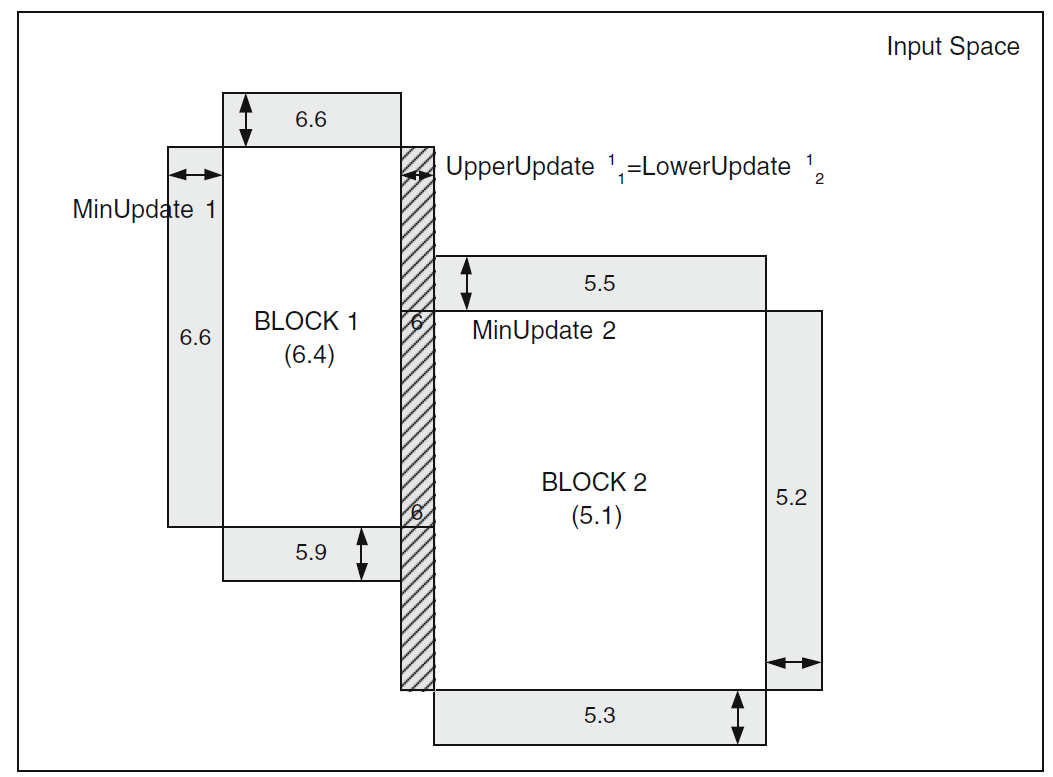
\includegraphics[width = \columnwidth]{img/cubes.png}
		\column{0.48\linewidth}
			\centering
			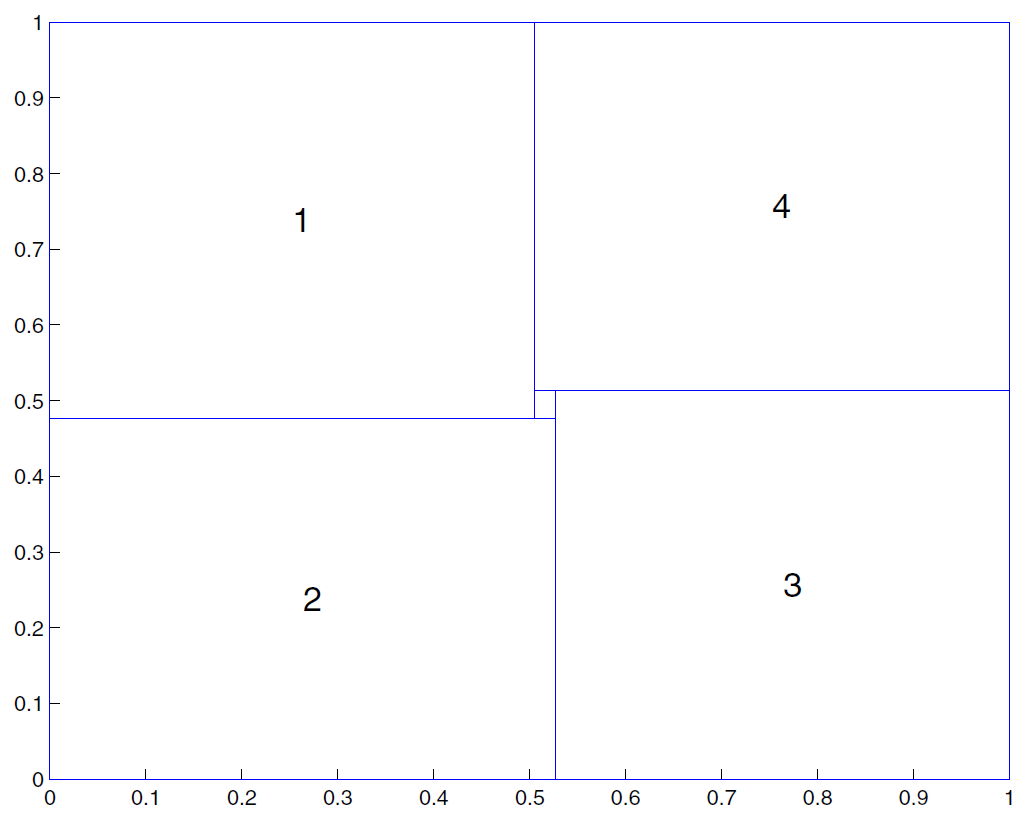
\includegraphics[width = \columnwidth]{img/iter.png}
	\end{columns}
	\centering
	Hyper-cubes creation and expansion in the \iter algorithm, images from \ccite{huysmans2006iter}
\end{frame}
%\\\\\\\\\\\\\\\\\\\\\

\begin{frame}
\frametitle{\gridex design}
	\begin{columns}[t]
		\column{0.33\linewidth}
			\centering
			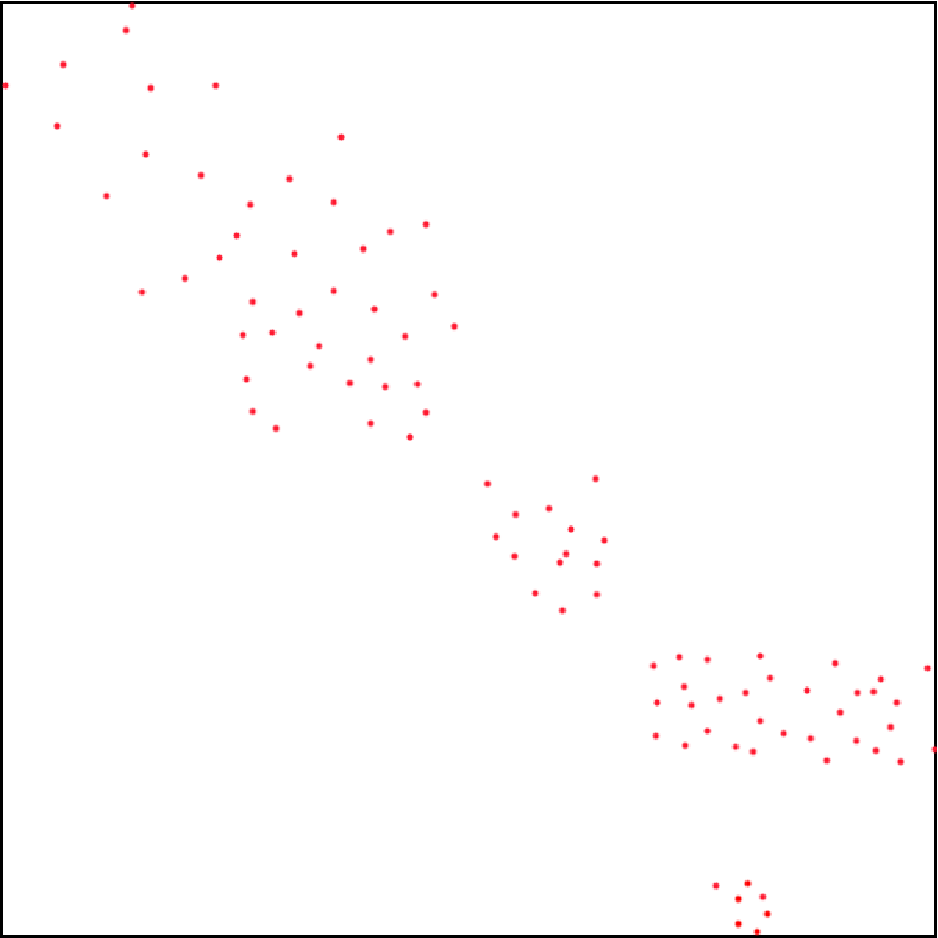
\includegraphics[width = \columnwidth]{img/demo/1.pdf}\\
			\scriptsize Input space and samples
		\column{0.33\linewidth}
			\centering
			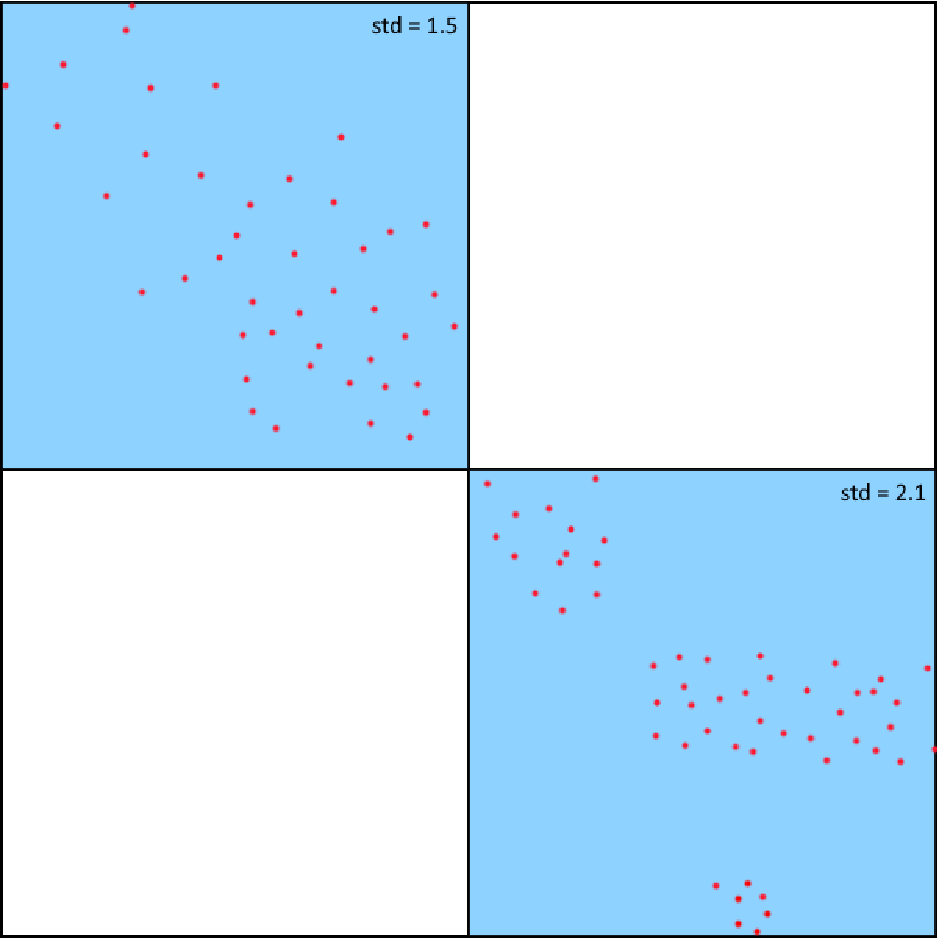
\includegraphics[width = \columnwidth]{img/demo/2.pdf}\\
			\scriptsize First split, with $p_1=2$
		\column{0.33\linewidth}
			\centering
			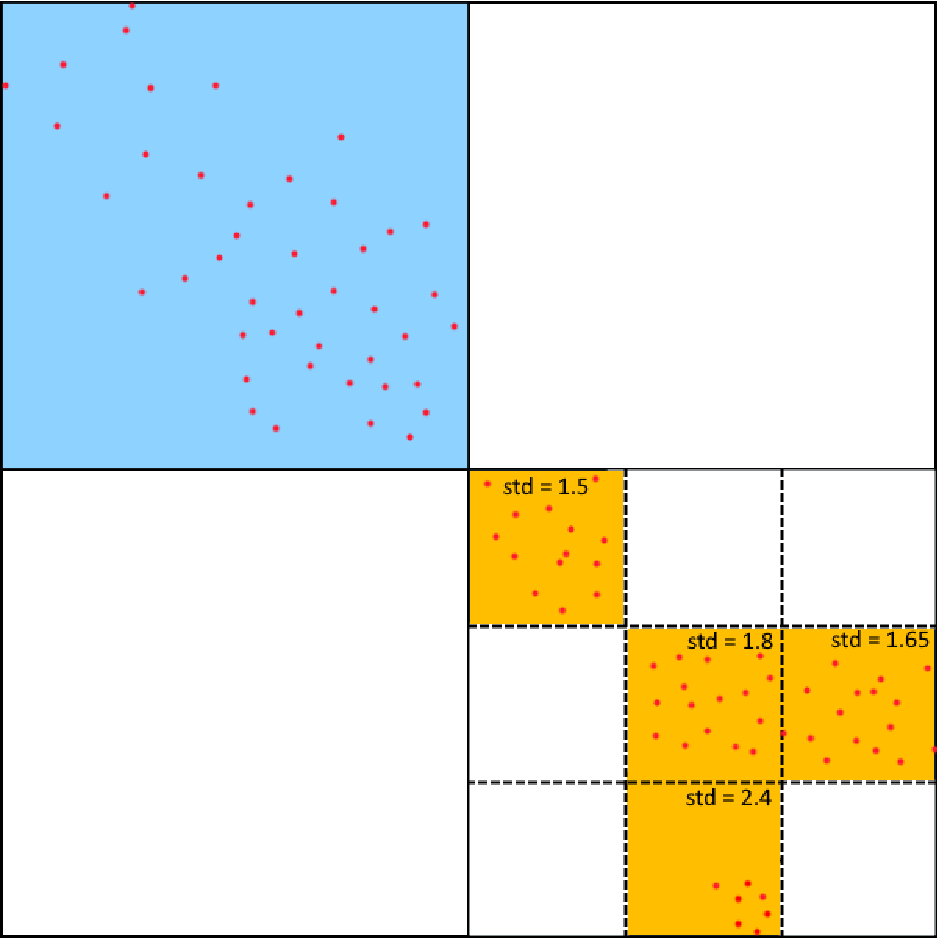
\includegraphics[width = \columnwidth]{img/demo/3.pdf}\\
			\scriptsize Second split, with $p_2=3$
	\end{columns}
	\centering
	\vspace{10px} \gridex recursive input space splitting
\end{frame}

\begin{frame}
\frametitle{Differences between \iter and \gridex}
	\begin{block}{
		\begin{tabular}{p{0.45\textwidth}p{0.25\textwidth}p{0.25\textwidth}}
			& \iter & \gridex
		\end{tabular}
	}
		\begin{tabular}{p{0.45\textwidth}p{0.25\textwidth}p{0.25\textwidth}}
			Approach & bottom-up & top-down \\
			Extracted rules & if-then-else & if-then-else \\
			Input region importance & no & yes \\
			Input feature importance & no & yes \\
			Input space coverage & non-exhaustive & exhaustive \\
			Suitable with few input features & yes & yes \\
			Suitable with many input features & no & yes \\
			Output value & constant & constant 
		\end{tabular}
	\end{block}
\end{frame}

\section{Experiments \& Results}

%\\\\\\\\\\\\\\\\\\\\\
\begin{frame}%[allowframebreaks]
\frametitle{Case study}

    \begin{itemize}
    	\item \gridex performance tested w.r.t. \iter and decision tree regressors
    	\begin{itemize}
    		\item in order to have neutral benchmarks
    	\end{itemize}
    
    	\vfill
    	
    	\item Several data sets of growing dimensionality
    	 \begin{itemize}
    		\item from 2 to 11 input features
    	\end{itemize}
    
    	\vfill
    	
    	\item Results averaged upon 10 executions for each data set
    	
    	\vfill
    	
    	\item Metrics: number of extracted rules, MAE and R$^2$ value
    	\begin{itemize}
    		\item with respect to both the underlying predictor and the actual data
    	\end{itemize}
    	
    	\vfill
    	
    	\item Selection of the best algorithm parameters
    	\begin{itemize}
    		\item considering the trade-off between fidelity and readability (\# of rules)
    	\end{itemize}
    	
    	\vfill
    \end{itemize}

\end{frame}

\begin{frame}%[allowframebreaks]
	\frametitle{Results}
	
	\begin{columns}
		\begin{column}{0.5\linewidth}
			Focus on:
			\begin{itemize}
				\item number of rules
				\item predictive performance w.r.t. the data
				\item fidelity w.r.t. the underlying predictor
				\item input space coverage
				\begin{itemize}
					\item \iter: 100\% only for simple data sets
					\item[$\rightarrow$] incomplete training sample coverage
					\item[$\rightarrow$] inability to predict every test sample
				\end{itemize}
			\end{itemize}
		\end{column}
		\begin{column}{0.5\linewidth}
			\centering
			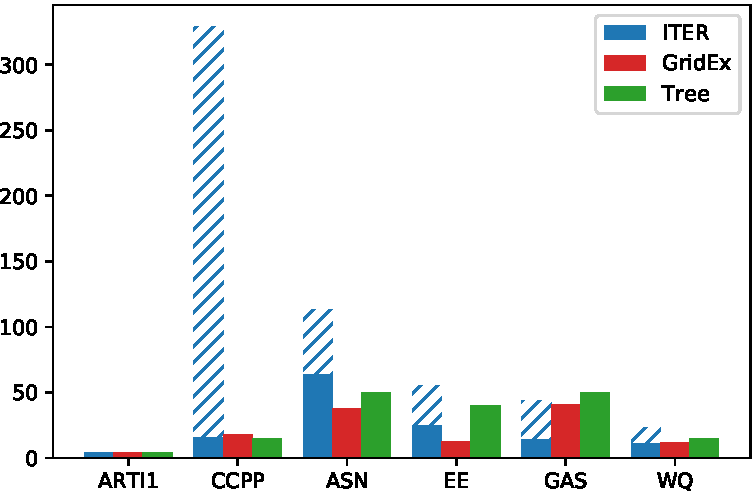
\includegraphics[width=\columnwidth]{img/comp/rules.pdf}
			\\
			\scriptsize Number of extracted rules
		\end{column}		
	\end{columns}	
\end{frame}

\begin{frame}%[allowframebreaks]
	\frametitle{Results}
	\scriptsize
	\begin{columns}[t]
		\column{0.5\linewidth}
			\centering
			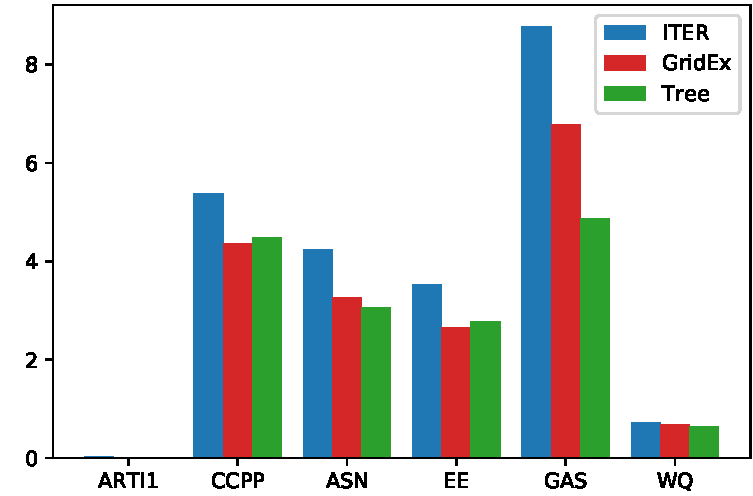
\includegraphics[width=.8\columnwidth]{img/comp/mae.pdf}\\
			MAE w.r.t. the data\vspace{10px}
			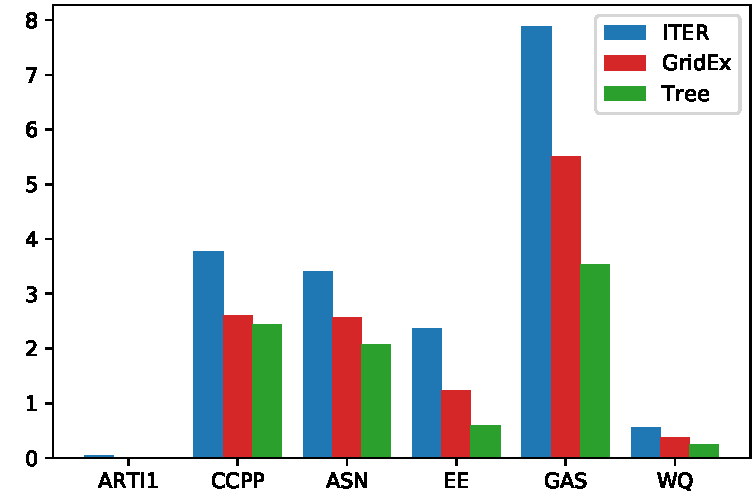
\includegraphics[width=.8\columnwidth]{img/comp/maefid.pdf}\\
			MAE w.r.t. the underlying black box
		\column{0.5\linewidth}
			\centering
			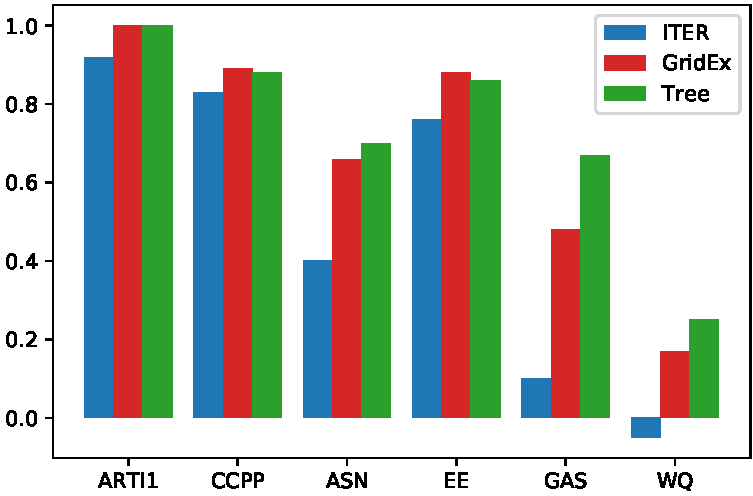
\includegraphics[width=.8\columnwidth]{img/comp/r2.pdf}\\
		 	R$^2$ value w.r.t. the data\vspace{10px}
			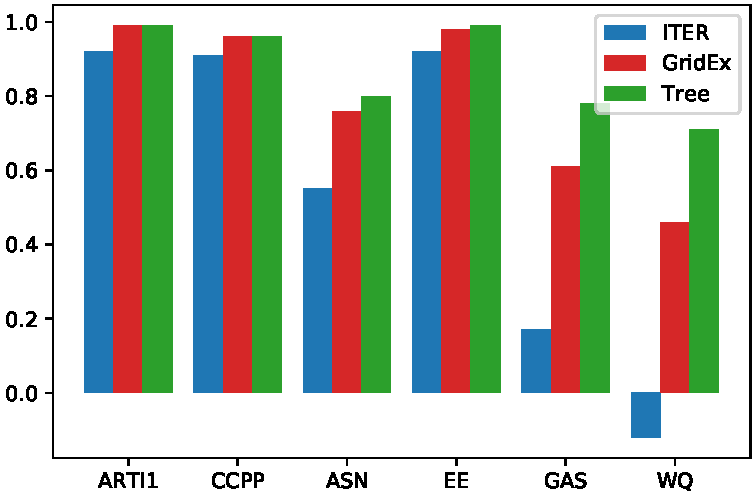
\includegraphics[width=.8\columnwidth]{img/comp/r2fid.pdf}\\
			R$^2$ value w.r.t. the underlying black box
	\end{columns}

	%	\subfloat[Number of extracted rules.]{
		%\subfloat[MAE with respect to the data.]{
		%\subfloat[MAE fidelity with respect to the underlying black box.]{
%		\subfloat[R$^2$ value with respect to the data.]{
		%\subfloat[R$^2$ value with respect to the underlying black box.]{
\end{frame}
%\\\\\\\\\\\\\\\\\\\\\

\section{Conclusions}

%\\\\\\\\\\\\\\\\\\\\\
\begin{frame}%[allowframebreaks]
\frametitle{Conclusions}

\begin{block}{Summing up}
	The new \gridex algorithm is able to:
    %
    \begin{itemize}
        \item overcome the \iter non-exhaustivity
        \item focus only on the interesting regions of the input space
        \item assign different weights to the input features
        \item produce shorter rule lists than \iter
        \item attain better predictive performances then \iter
        \item simplify the parameter tuning phase
    \end{itemize}
\end{block}

\end{frame}

\begin{frame}
	\frametitle{Future works}

\begin{exampleblock}{Future works}
	Our next research efforts will be focused on:
	\begin{itemize}
		\item overcoming the remaining limitations of \iter and other algorithms
		\begin{itemize}
			\item[e.g.] address the inability to handle categorical features
			\item[e.g.] substitute the constant output value of the produced decision rules
		\end{itemize}	
		\item the enhancement of \gridex
	    \begin{itemize}
			\item[e.g.] automatise the adaptive split thresholds of \gridex
		\end{itemize}		
	\end{itemize}
\end{exampleblock}

\end{frame}
%\\\\\\\\\\\\\\\\\\\\\

%===============================================================================
\section*{}
%===============================================================================
\frame{\titlepage}

%===============================================================================
\section*{\bibname}
%===============================================================================

\setbeamertemplate{page number in head/foot}{}
%\\\\\\\\\\\\\\\\\\\\\
\begin{frame}[t,allowframebreaks,noframenumbering]\frametitle{\refname}
% \begin{frame}[c]\frametitle{\refname}
	\footnotesize
%	\scriptsize
    \bibliographystyle{plain}
	\bibliography{SCO-EXTRAAMAS-2021-talk}
\end{frame}
%\\\\\\\\\\\\\\\\\\\\\

%%%%%%%%%%%%%%%%%%%%%%%%%%%%%%%%%%%%%%%%%%%%%%%%%%%%%%%%%%%%%%%%%%%%%%%%%%%%%%%%
\end{document}
%%%%%%%%%%%%%%%%%%%%%%%%%%%%%%%%%%%%%%%%%%%%%%%%%%%%%%%%%%%%%%%%%%%%%%%%%%%%%%%%
